\documentclass{../style/sig-alternate}

\usepackage{here}

%----------- マクロ ----------
%数式番号を節毎に分けてリセットする
\def\theequation{\thesection.\arabic{equation}}
  \makeatletter
  \@addtoreset{equation}{section}
  \makeatother
%図番号を節毎に分けてリセットする
\makeatletter
 \renewcommand{\thefigure}{%
   \thesection.\arabic{figure}}
  \@addtoreset{figure}{section}
\makeatother
%表番号を節毎に分けてリセットする
\makeatletter
 \renewcommand{\thetable}{%
   \thesection.\arabic{table}}
  \@addtoreset{table}{section}
\makeatother

\makeatletter
 \let\@copyrightspace\relax
 \makeatother

\begin{document}

\title{SLSTC at the NTCIR-12 Task}

\numberofauthors{5}
\author{
% You can go ahead and credit any number of authors here,
% e.g. one 'row of three' or two rows (consisting of one row of three
% and a second row of one, two or three).
%
% The command \alignauthor (no curly braces needed) should
% precede each author name, affiliation/snail-mail address and
% e-mail address. Additionally, tag each line of
% affiliation/address with \affaddr, and tag the
% e-mail address with \email.
%
% 1st. author
\alignauthor
Hiroto Denawa\\
       \affaddr{Waseda University}\\
       \email{hi\_denawa@fuji.waseda.jp}
% 2nd. author
\alignauthor
Tomoaki Sano\\
       \affaddr{Waseda University}\\
       \email{tonosamoaki@asagi.waseda.jp}
\and  % use '\and' if you need 'another row' of author names
% 3rd. author
\alignauthor
Yuta Kadotami\\
       \affaddr{Waseda University}\\
       \email{kdtm-783640@ruri.waseda.jp}
% 4th. author
\alignauthor
Sosuke Kato\\
       \affaddr{Waseda University}\\
       \email{sow@suou.waseda.jp}
%\and  % use '\and' if you need 'another row' of author names
% 5th. author
\alignauthor
Tetsuya Sakai\\
       \affaddr{Waseda University}\\
       \email{tetsuyasakai@acm.org}
}

\maketitle

\begin{abstract}
The SLSTC team participated in the Short Text Conversation (STC) subtask of the NTCIR-12 Mission Impossible Task.
This minority report describes our approach to solving the STC problem and will discuss the official results.
\end{abstract}

\section*{Team Name}
SLSTC

\section*{Subtasks}
Short Text Conversation (Japanese)

\keywords{STC,HNN,Word2Vec,Subnetwork}

\section{Introduction}

SLSTC (The Sakai Laboratory, Waseda University) participated in the
Japanese subtask of the STC task.
This paper briefly describes our approaches,
and reports on the official results.

Table \ref{tab:run_list}  shows the list of runs that we submitted to the STC Japanese subtask.
In Section~\ref{sec:methods}, we describe the algorithms we employed
to generate these runs.
In Section~\ref{sec:results}, we discuss the official results of our runs.
Finally, in Section~\ref{sec:conclusions}, we conclude this paper
and lists up future work items.

\begin{table}[h!]
  \centering
  \caption{the list of runs}
  \label{tab:run_list}
  \begin{tabular}{|c|} \hline
     run name \\ \hline
     SLSTC-J-R1 \\ \hline
     SLSTC-J-R2 \\ \hline
     SLSTC-J-R3 \\ \hline
  \end{tabular}
\end{table}

\section{Methods}
\label{sec:methods}

\subsection{SLSTC-J-R1}

This experiment can be divided in following 4 parts: 1st parts of generating distributed representation, 2nd of processing train data, 3rd of training and 4th of applying system learned and evaluation. In this section details of these are shown below.

\subsubsection{Distributed Representation Generating Part}

There is a tool for generate distributed representation of words called Word2Vec\cite{word2vec}.
Word2Vec is announced by Google in 2013 and attracted researchers’ attention all over the world.
Input a corpus, Word2Vec generates vectors for each word in the corpus.
Words which have close meaning have close vectors to each other.
In this research, Wikipedia in Japanese and Nicopedia (Niconico Daihyakka in Japanese) corpus were used to generate distributed representation, to apply to somehow casual representation in sentences.

\subsubsection{Train Data Processing Part}

Dataset is provided by NTCIR-12 STC Task.
From this dataset, 427200 pairs of post tweet and reply tweet were obtained (maybe some were deleted).
For each tweet in this dataset, morpheme analysis was done by using MeCab\cite{mecab}.
Then, for each tweet, vector representation of it was calculated as follows.
$ i $ th morpheme in tweet $ t $ was defined as  and its vector (distributed) representation is noted as $ {\bf w_{i,t}} $.
The vector representation of tweet $ t $ is calculated by:

\begin{eqnarray}
 {\bf t} = \sum_{i=1}^{|t|} tfidf(w_{i,t}) \cdot {\bf w_{i,t}} \cdot f(t,i)
\end{eqnarray}

Note that $ f(t,i) = e^{\frac{|l|}{i}} $ if $ i $ th morpheme in $ t $ is content word and  if otherwise.
This is to emphasize weight of content words.

\subsubsection{Learning Part}

In this research, process to make valid reply for given post is considered as a translation by Hierarchical Neural network (HNN) , which has 3 layers.
In this part, weight matrices in the HNN is learned by Error Back Propagation method\cite{bahman}.
The parameters used in this part are shown in table \ref{tab:hnn_parameters} below.
Note  stands for the sigmoid function .

\begin{table}[h!]
  \centering
  \caption{Parameters for learning}
  \label{tab:hnn_parameters}
  \begin{tabular}{|c|c|} \hline
     {\bf Parameters} & {\bf Value} \\ \hline
     Dimension of input layer & 200 \\ \hline
     Dimension of hidden layer & 100 \\ \hline
    Dimension of output layer & 200 \\ \hline
    Activity function to hidden & $ \sigma ( x ) $ \\ \hline
    Activity function to output & $ 2 \sigma ( x ) - 1 $ \\ \hline
    Learning efficiency $ \eta $ & $ 1.0 \times 10^{-4} $ \\ \hline
    Error threshold & $ 1.25 \times 10^{-2} $ \\ \hline
  \end{tabular}
\end{table}

This model is tested in 3-cross evaluation method.
All data were divided into 3 groups and tested in the scheme shown in table \ref{tab:testing_scheme} below.

\begin{table}[h!]
  \centering
  \caption{Training and testing scheme}
  \label{tab:testing_scheme}
  \begin{tabular}{|c|c|c|c|} \hline
     {\bf Experiment No.} & 1 & 2 & 3 \\ \hline
     {\bf Group No.} & & & \\ \hline
     0 & \multicolumn{2}{|c|}{Train} & Test \\ \hline
    1 & Test & \multicolumn{2}{|c|}{Train} \\ \hline
    2 & Train & Test & Train \\ \hline
  \end{tabular}
\end{table}

\subsubsection{Applying and Evaluating Part}
\label{sec:applying}

For each posts in each test case, five reply candidates, which has from 1st to 5th smallest error to its output are suggested.

\begin{figure}[h!]
 \begin{center}
  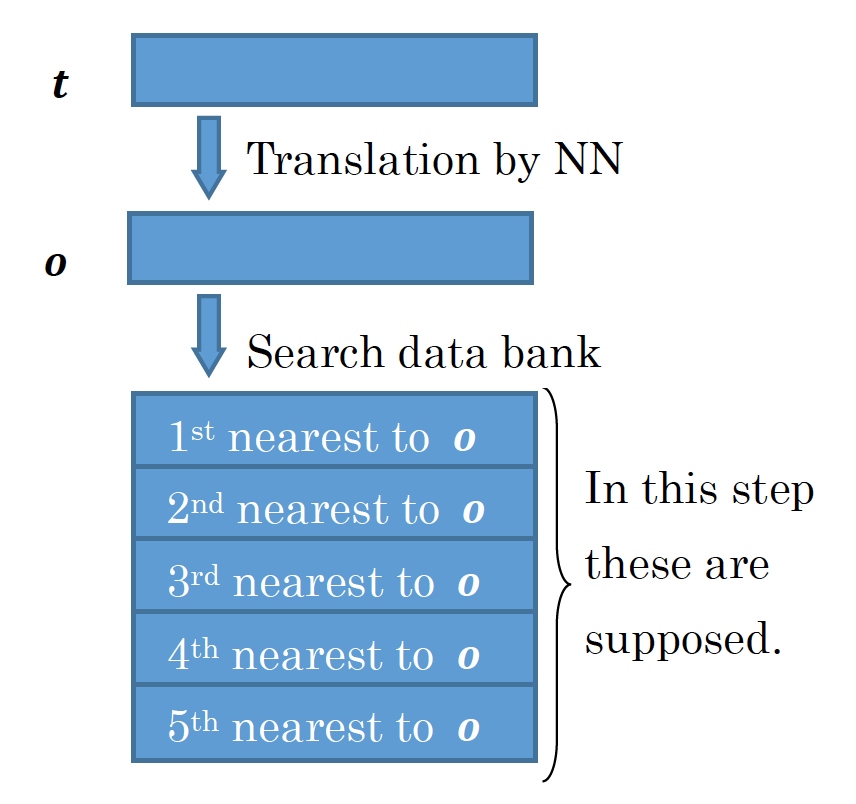
\includegraphics[width=120mm,bb=0 0 616 579]{../img/peter_fig01.png}
  \end{center}
  \caption{description of step}
  \label{fig:applying}
\end{figure}

\subsection{SLSTC-J-R2 and SLSTC-J-R3}

\section{Official Results and Discussions}
\label{sec:results}

\section{Conclusions and Future Work}
\label{sec:conclusions}

\begin{thebibliography}{99}

%\bibitem{sakai} Sakai, T., Shang, L., Lu, Z. and Li, H.: Topic Set Size Design with the Evaluation Measures for Short Text Conversation, AIRS 2015, LNCS 9460, pp.1-13, 2015.
\bibitem{word2vec} Google Word2Vec, https://code.google.com/p/word2vec/
\bibitem{mecab} MeCab, http://taku910.github.io/mecab/
\bibitem{bahman} Bahman Kermanshahi, Construction and Application of Neural Network,Shokodo

\end{thebibliography}


\end{document}
